\documentclass[a4paper]{article}

\usepackage{cite}
\usepackage[english]{babel}
\usepackage[utf8]{inputenc}
\usepackage{amsmath}
\usepackage{graphicx}
\usepackage[colorinlistoftodos]{todonotes}

\title{Using Lattice Boltzmann Methods to Simulate Flows in Complex Geometries}

\author{Zachary Sustiel}

\date{\today}

\begin{document}
\maketitle


\section{Introduction}
A fluid is characterized by continuous macroscopic fields obtained by coarse graining over local particles at each position in space, and the corresponding gas dynamics may then be described by a set of continuity equations and an equation of state. Many situations arise in hydrodynamics in which no analytic solution to these equations exists, and consequently the flow must be solved numerically. One common such method is to simply discretize the constitutive equations and use numerical methods to solve for the system dynamics.

This method is inherently macroscopic, in the sense that we simply solve the Navier Stokes equations without any information about the microdynamics of the system. The purpose of this report shall be to introduce an alternative, mesoscopic method known as the Lattice Boltzmann method, and discuss its applicability towards computational hydrodynamics. 

Perhaps the greatest benefit of the LBM is that it is massively parallelizable, making it optimal for GPU computation or parallel computing clusters. \footnote{Another noteworthy aspect of the Lattice Boltzmann method is a sort of "dual-functionality" which arises as a result of implementing both macroscale and microscale interactions. In addition to the so-called "bottom-up" approach in which fluid dynamics are simulated by numerically by solving for the system microdynamics,  there also exists a so-called "top-down" approach in which microdynamics are studied by using the LBM to measure microscopic relaxation times. \cite{latticehistory} Here, of course, we concern ourselves with the former.} Our primary focus, however, will be using Lattice Boltzmann methods to study flows in complex geometries.

The structure of this report is as follows. To preface our explanation of the Lattice Boltzmann Method, we first discuss the Boltzmann Equation and the BGK collision operator, and introduce the Lattice Gas Automata. Next, we discuss the Lattice Boltzmann Method, and outline a D2Q9 algorithm which we implement in python. We then discuss boundary conditions; namely, we discuss halfway and fullway bounce-back boundaries, as well as Zou-He boundaries. Finally, we present the results of a series of benchmark tests using the Lattice Boltzmann Method:
\begin{enumerate}
    \item We generate a Poisseuille flow by setting up a pressure gradient in a channel with no-slip walls, and compare the computed velocity profile to the analytical incompressible solution.
    \item Using momentum exchange, we attempt to evaluate the force exerted on the channel walls by the fluid
    \item We simulate the flow around a cylinder embedded in a Poisseuille flow at both high and low Reynolds numbers, and try to observe vortex shedding in the turbulent regime
    \item We present a flow around a complex boundary
\end{enumerate}

The research done in this project is not ground breaking: the algorithms which we use are widely known and relatively low order, and the series of benchmark simulations (generating pressure-driven flow, modeling the flow around a cylinder, and calculating lift and drag forces using momentum exchange) are all simple, straightforward to implement, and have been studied to death. Instead, this project serves as an instructive exercise as well as a proof of concept. We seek to demonstrate that Lattice Boltzmann Methods are able to simulate flows in complex geometries with reasonable accuracy and relatively little effort, which is rather remarkable in and of itself. For instance, as we shall discuss, though the particular scenario of the flow around a cylinder is well-understood, we may just as easily model the flow around an object of nontrivial shape (say, a peanut) with minimal effort. Provided slightly  more refined methods for force evaluation and boundary interactions were implemented, it is reasonable to assume one may calculate the drag and lift forces on an obstacle of any shape in a flow; a non-trivial result with physical, real-world implications. Consequently, in this project we do not present ground-breaking results, but instead insist that the Lattice Boltzmann Method which we present can be used to achieve substantial results in the future. 

\section{Theory}

\subsection{Lattice Gas Automata}
The Lattice Gas Automata is a simplified model of gas dynamics in which a small number of "representative" particles are confined to move along a lattice. Reducing the number of particles and severely restricting their trajectories in this manner drastically reduces the number of calculations needed to keep track of microscopic positions, velocities and collisions.

The D2Q9 model restricts the particle positions $\vec{x_i}$ to the nodes of a 2D lattice, and the microscopic velocities $u_i$ such that after each timestep a particle either remains stationary or moves to one of the eight adjacent nodes. Consequently, particles may have one of nine discreet velocities $\vec{e_i}, i \in \{0, 1, 2, 3, 4, 5, 6, 7, 8, 9\}$, which correspond to the nine directions which a particle may "stream" as illustrated in Figure (1) below \cite{meskas}. When two particles stream to the same lattice site, they collide according to standard conservation of momentum.  

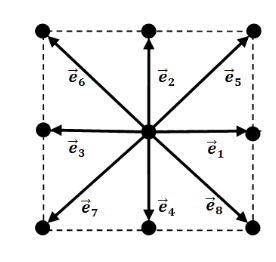
\includegraphics[width=5cm]{meskas_1.PNG}

A microscopic method like the LGA has advantages and disadvantages compared to the standard macroscopic hydro code. A great advantage is that the streaming step is incredibly parallelizable, since the position of each particle after streaming does not depend on the position of any other particles. Consequently, the streaming step is optimal for GPU computation or parallel computing clusters, as communication between cores is only necessary to complete the collision step. 

The LGA also excels in computing flows around boundaries with complex geometries. For instance, solving the density, velocity and pressure fields for a flow around an oddly-shaped object can be complicated, especially if the object has no exploitable symmetries. On the other hand, in the LGA, such a boundary is trivial: when a particle encounters a boundary node, it simply collides with the object according to momentum conservation. As we shall see in the Lattice Boltzmann Method, the force exerted on an object by a flow can be computed in a similar manner. 

The main drawback of the LGA is that it suffers from high statistical noise\cite{latticehistory}; the dynamics of the particles confined to a lattice only roughly approximate the dynamics of a physical, unrestrained gas. The Lattice Boltzmann Method remedies this by streaming ensemble averages instead of literal particles, and consequently is often more popular than the standard LGA.\footnote{A more detailed comparison of the LGA and LBM, and a brief history on the development and relation of the two methods, is given in Li-Shi Luo's "The Future of Lattice-Gas and Lattice Boltzmann Methods"}

\subsection{Lattice Boltzmann Method}
In the Lattice Boltzmann Method (LBM), the representative particles of the LGA are replaced by the particle distribution function $f(\vec{x}, \vec{v}, t)$, or the probability of finding a particle at position $\vec{x}$ with velocity $\vec{v}$ at time $t$. The system dynamics can then be obtained from the Boltzmann Equation \footnote{The Boltzmann Transport Equation and the BGK Collision Operator are likely discussed in further detail in many higher-level statistical mechanics textbooks, such as Chapter 3 of Mehran Kardar's "Statistical Physics of Particles".},
\begin{equation}
    \frac{\partial f}{\partial t} + \vec{u}\cdot \vec{\nabla} f + \frac{F}{m}\frac{\partial f}{\partial \vec{u}} = \frac{1}{\tau}(f^{eq} - f)
\end{equation}
where $u$ is the microscopic velocity, $m$ is particle mass, and $\vec{F}$ is external force. The two leftmost terms correspond to particle streaming, and the expression on the right hand side corresponds to the BGK collision operator, with a relaxation time $\tau$ which we will discuss in more detail shortly.

In the case of the D2Q9 model, in which microscopic velocities are restricted to a discrete set, we may introduce new particle distribution functions $f_i(\vec{x}, t) = f(\vec{x}, \vec{e}_i, t)$. The macroscopic density $\rho$ and velocity $\vec{v}$ are easily recovered via ensemble averages, which are reduced to the discrete sums;

\begin{align}
    \rho(\vec{x}, t) &= \sum_{i=0}^8 f_i(\vec{x}, t) \\
    \vec{v}(\vec{x}, t) &= \frac{1}{\rho} \sum_{i=0}^8 c\vec{e}_i f_i(\vec{x}, t) 
\end{align}

In the absence of external forces, the discretized Boltzmann equation is 
 \begin{equation}
     f_i(\vec{x} + \vec{e}_i\Delta t, t + \Delta t) = f_i(\vec{x}, t) + \frac{\Delta t}{\tau}\Big(f_i^{eq}(\vec{x}, t) - f_i(\vec{x}, t)\Big) 
 \end{equation}
 
The term $f_i^{eq}(\vec{x}, t)$ corresponds to the local equilibrium distribution at a position $\vec{x}$ and time $t$, and depends on the macroscopic density and velocity $\rho(\vec{x}, t)$ and $\vec{v}(\vec{x}, t)$ as
\begin{equation}
    f_i^{eq} = \rho\omega_i\Big(1 + 3\vec{e}_i\cdot\vec{v} + \frac{9}{2}(\vec{e}_i\cdot\vec{v})^2 - \frac{3}{2}(\vec{v}_i\cdot\vec{v})^2\Big)
\end{equation}
where the weights $\omega_i$ are 
\begin{equation}
    \omega_i = \left\{\begin{array}{cl}
        4/9, & i = 0 \\
        1/9, & i = 1, 2, 3, 4 \\
         1/36, & i = 5, 6, 7, 8
    \end{array}\right.
\end{equation}

The standard LBM algorithm \footnote{The algorithm given here was presented in \cite{meskas}. This algorithm is relatively standard, with slight variation. For instance, in our implementation, we choose to perform the collision step before the streaming step instead of afterwards, without loss of generality.} is relatively straightforward: 

\begin{enumerate}
    \item Initialize $f_i, f_i^{eq}, \rho,$ and $\vec{v}$ 
    \item Compute the the streaming term $f_i^*$ by moving $f_i$ in the direction $\vec{e}_i$; i.e. $f_i^*(\vec{x} + c\vec{e}_i\Delta t, t + \Delta t) = f_i(\vec{x}, t)$ 
    \item Calculate the macroscopic fields $\rho$ and $\vec{v}$ using $f_i^*$  
    \item Use the macroscopic fields to calculate $f_i^{eq}$
    \item Compute the collision term to find the updated distribution function $f_i(\vec{x}, t + \Delta t) = f_i^*(\vec{x}, t) + \frac{\Delta t}{\tau}\big(f_i^{eq}(\vec{x}, t) - f_i^*(\vec{x}, t)\big)$
    \item Repeat streaming and collision steps 
\end{enumerate}

Note that even though the LBM uses probability distribution functions, this method is entirely deterministic. Just as macroscopic quantities are determined by coarse-graining in hydrodynamic models, the macroscopic fields are recovered by the $f_i$ in the same manner, and the $f_i$ are treated using finite difference methods. In fact, the LBM can be viewed as a finite difference equation for solving the Boltzmann Equation on a lattice, and one of the primary reasons that LBM's can be used for fluid simulations is that the Navier Stokes equations can be recovered from the discrete equations. \cite{meskas, acoustics, buk}

\subsection{Unit Conversion, Stability and Viscosity}
The description of our LBM model so far been entirely in lattice units, but have not described any connection between LBM fluid simulations and physical flows. A physical length scale $L$ is introduced into our model via the grid spacing $h \equiv L/N$ - where $N$ is the number of nodes spanned by a length $h$ - and physical quantities are related to lattice parameters through the spacial resolution $h$ and the timestep $s$. For instance, the physical velocity is given by $\Tilde{\vec{v}} = \frac{h}{s}\vec{v}$, and the physical speed of sound is $\Tilde{c_s} = \frac{h}{s}c_s = \frac{1}{\sqrt{3}}\frac{h}{s}$. Dimensional analysis in this manner can be used more generally to convert between lattice units and physical units. \cite{acoustics} 

The viscosity of the fluid is given by 
\begin{equation}
    \nu = c_s^2(\tau-\frac{1}{2})\frac{h^2}{s}
\end{equation}
The significance of $\nu$ is twofold. First, we may rewrite the expression for viscosity to obtain an expression for the timestep in lattice units:
\begin{equation}
    s = c_s^2h^2\frac{\tau - \frac{1}{2}}{\nu}    
\end{equation}
where for a fixed viscosity $\nu$, the relaxation time $\tau$ is the only free variable. Second, we note that we may also rewrite this in terms of physical units by replacing $c_s$ by $\Tilde{c_s}$, and solving for $s$ gives the equivalent expression
\begin{equation}
    s = \frac{1}{\Tilde{c_s^2}}\frac{\nu}{\tau - \frac{1}{2}}    
\end{equation}
From the second equation, we see that the timestep is restricted by $\tau > 0.5$, and there is an instability at $\tau = 0.5$. \cite{meskas, acoustics} This restriction limits the efficiency of the BGK collision operator, and for this reason many opt to use a collision operator of a different form, such as a multiple relaxation time implementation. \cite{multirelaxtimes} However, the BGK operator is sufficiently stable for our purposes.

Further, it is clear from the above expressions that we are justified to fix the relaxation time $\tau = 1.0$ and instead vary viscosity as the free variable. In this manner, we opt to ignore $\tau$ completely and instead adopt an intuitive interpretation that our timestep is inversely proportional to the fluid viscosity, and instabilities arise as viscosity goes to zero.

We then keep in mind that our simulation degrades for very low viscosity; however, as we shall see, we can still simulate viscous laminar flows with first or second order accuracy in space.

\subsection{Boundaries}
For a standard fluid node with eight adjacent nodes, all nine $f_i$ are known after streaming. This is not the case for boundary nodes, which do not have a complete set of adjacent knowns. For instance, a node on the lefthand edge of the lattice will have $f_1, f_5,$ and $f_8$ undetermined after streaming because these $f_i$ come from points which lie outside of the lattice. Consequently, the values to the unknown $f_i$ correspond to the macroscopid boundary conditions which we choose to enforce.

\subsubsection{No-Slip: Half and Full Bounce-Back, Embdedded Objects and Force Evaluation via Momentum Exchange}
Perhaps the easiest and most common boundary condition is the bounce-back method. At any boundary node, we simply assign \begin{equation}
    f_i = f_i^-
\end{equation}
for each $f_i$, where $f_i^-$ is the particle distribution function corresponding to the opposite direction ($f_1^- = f_3, f_5^- = f_7$, etc.) Recalling that macroscopic velocity is determined by Equation (3), it is clear that the bounce-back method give $\vec{v} = 0$ at the walls. 

There are several ways that bounce-back boundaries may be implemented. The simplest is on-grid bounce back, in which the boundaries coincide with the walls. Despite only first order accurate in space, on-grid implementations are frequently used due to their sheer simplicity. A second order bounce-back method exists in which ghost cells are initialized outside of the fluid domain, and the wall instead is placed halfway between nodes rather than coinciding with the lattice nodes. Furthermore, the reversal of $f_i$'s may be carried out either during the collision step or during the streaming step. For the highest accuracy, we always execute bounce-back during the streaming step, and choose to implement the "halfway" bounce-back method, in which the walls are placed halfway between nodes. The increase from first to second order accuracy, is a consequence both of the centered nature of the halfway bounce-back method, as well as the fact that the collision step is also executed on the boundary nodes.

The force exerted on the boundary is also easily calculated by the momentum-exchange method \cite{momentumexchange} \cite{forcedcurved}. The change in momentum, and consequently the force on the boundary, is simply
\begin{equation}
    F_i = e_i(f_i^{*-} + f_i) 
\end{equation}

\subsection{Zou He: Pressure Driven Flow, Poisseuille-Like Flow}
To enforce nonzero velocity or constant pressure at the boundary, we use Zou-He boundary conditions. For instance, at a channel inlet or outlet, we assert that $v_y = 0$ and $\rho \propto P$ is constant, and so the values of the unknown $f_i$ are restricted by the sums from Equations (2) and (3). For a more detailed derivation, one may refer to \cite{ZouHe}. \cite{ZouHe} The unknown $f_i$ at the channel inlet are determined as follows \cite{ZouHe}:
\begin{align}
    v_x &= 1 - \frac{1}{\rho_L}\big(f_0 + f_2 + f_4 + 2(f_3 + f_6 + f_7)\big), \nonumber \\
    f_1 &= f_3 + \frac{2}{3}\rho_Lv_x \nonumber\\
    f_5 &= f_7 - \frac{1}{2}(f_2 - f_4) + \frac{1}{6}\rho_Lv_x \nonumber\\
    f_8 &= f_6 + \frac{1}{2}(f_2 - f_4) + \frac{1}{6}\rho_Lv_x
\end{align}

\section{Results}
A D2Q9 Lattice Boltzmann Method was implemented in Python and used to simulate fluids on an $N$x$M$ lattice subject to various boundary conditions. We took $\tau=1$, $\nu = 25.0$, $L=40$, and $h=N/L$.

\subsection{Pressure-Driven Flow}
A pressure-driven flow through a no-slip channel was simulated using Zou-He boundary conditions to impose a pressure gradient across the system, and bounce-back boundary conditions to impose the no-slip condition at the channel walls. The analytic steady state solution for an incompressible fluid subject to these boundary conditions is known exactly as 
\begin{equation}
    \vec{v} = \frac{\rho_0\Delta P}{2\nu}y(H-y)\hat{x} 
\end{equation}
where $H = h*M$ is the channel height, and $\Delta P = P_L - P_R = \frac{1}{3}(\rho_L - \rho_R)$ is the difference between the outlet and inlet pressures. We took $\Delta P = 0.05$ and $\rho_0 = 1.0$, continued to iterate until the steady-state condition
\begin{equation}
    TOL \equiv \sum_{j=0}^{M-1} |v_x(y=j, t=t+s) - v_x(y=j, t=t)| < 10^-8
\end{equation}
had been satisfied. 

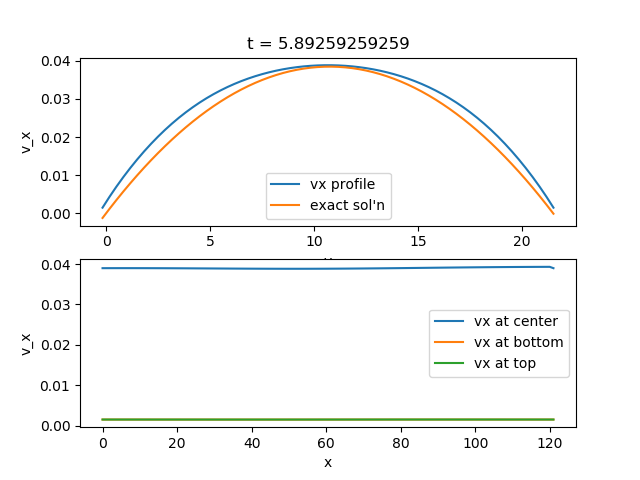
\includegraphics[width=12cm]{poisseuille_2.png}

The figure above illustrates various $v_x$ profiles. The top figure shows the computed $v_x$ profile in the $y$ direction (with $x = N/2$) in blue, as well as the exact solution in orange. It is clear that the calculated velocity profile differs slightly from the exact solution. This is because our model is not incompressible, which is illustrated by the fact that there is not invariance along the x direction. We would expect to see convergence if we instead were to implement the incompressible D2Q9i model \cite{ZouHe} or run the model at very low Mach number ($v << c_p = \frac{1}{3}\frac{h^2}{s^2}$). In other works this has been done to verify that the convergence rate of the bounce-back method agrees with theoretical predictions, and would be a nice benchmark task to pursue in the future. \cite{meskas}

The bottom velocity profile measures $v_x$ in the x direction both at the channel walls ($y=-1$ and $y = M$) and along the channel center $y = M/2$. These plots show that the velocity at the channel wall is significantly smaller than that at the channel center, suggesting that bounce-back conditions work with sufficient accuracy. 

\subsubsection{Force Evaluation}
The drag and lift forced exerted on the channel walls were measured using the Momentum Exchange Method for flows of various pressure gradients. The results are presented in the plot below. Force is shown only on the top wall, since the force on the bottom wall is calculated to have equal magnitude. 

\begin{center}
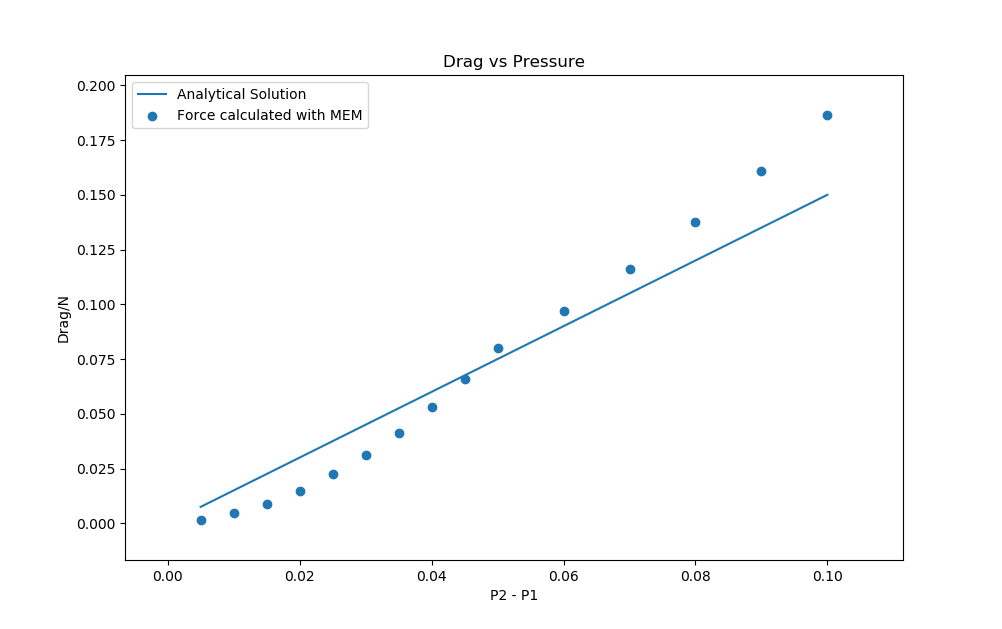
\includegraphics[width=12cm]{channel_2.png}
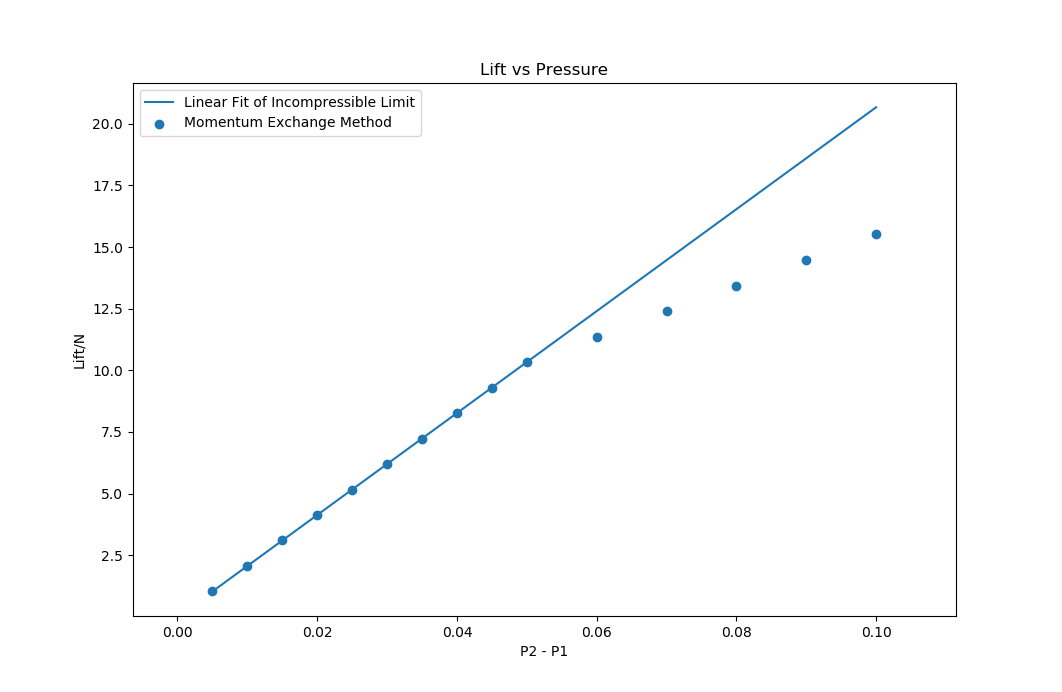
\includegraphics[width=12cm]{channel_1.png}
\end{center}

In the incompressible limit we expect both forces to increase linearly with velocity, which in the incompressible limit is proportional to the pressure gradient $dP$. The drag force increases somewhat linearly at low $dP$, and in a different manner at higher $dP$. The lift force (the force exerted perpendicular to the wall by the fluid) increases linearly at low $dP$, and increases differently at higher $dP$. There is a specific $dP$ at which both the drag and lift curves change behavior, indicating the possible existence of a critical point. I suspect this feature is related either to compressibility or to viscosity, but further study is needed to determine the significance of this point. 

\subsection{Flow around Embedded Objects}
The flow around a cylinder was studied, and plots of the computed streamlines are shown below. At $dP=0.05$ the system displays laminar flow around the cylinder consistent with theoretical predictions. Furthermore, as $dP$ is increased to simulate higher Reynolds number flow, the system forms a pair of vortices, as theoretically predicted. Another nice benchmark for the future would be to systematically increase the Reynolds even further to achieve vortex shedding. Furthermore, comparison with the theoretical Reynolds number at which vortex shedding has been observed experimentally can help verify the relationship between physical viscosity and numerical parameters described above. 
\begin{center}
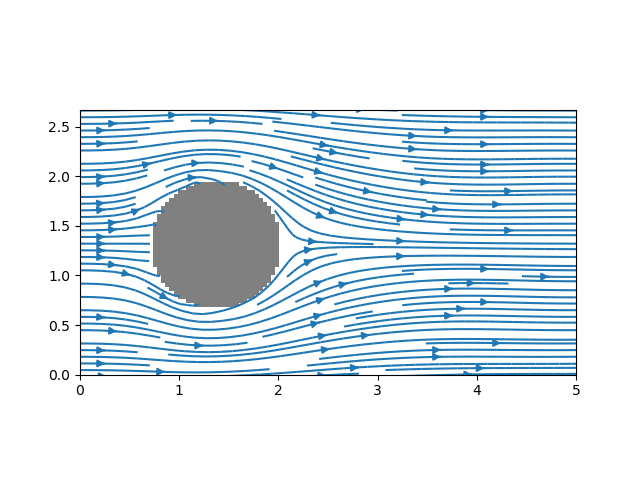
\includegraphics[width=10cm]{cyl.png}
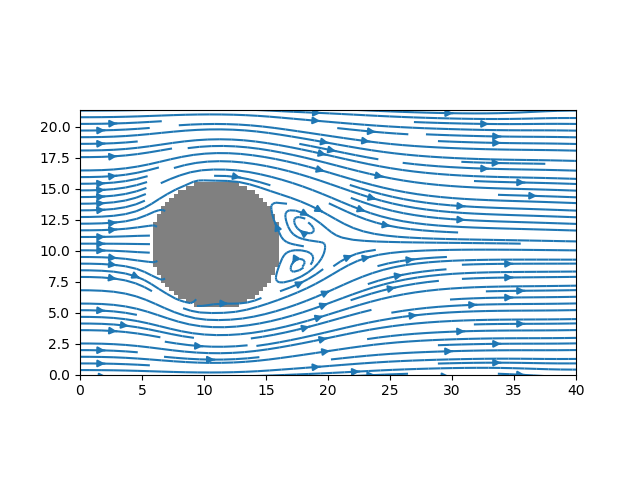
\includegraphics[width=10cm]{vortices.png}
\end{center}
Here we omit a force calculation of the drag and lift on a cylinder because the accuracy of the bounce-back method is degraded by the introduction of curved boundaries. Recall that the accuracy of the bounce-back method was improved from 1st order to 2nd order simply by shifting the wall from the boundary nodes to halfway between nodes. Likewise, circular boundaries intersect the lattice at various which are neither perfectly on nor halfway between nodes, and so the accuracy of the bounce-back method in this case is degraded accordingly. Although MEM is relatively easy to implement on an arbitrary boundary, the accuracy of such a calculation is degraded enough that it would be better to implement a different boundary method designed to handle curved boundaries to a given accuracy. 

\begin{center}
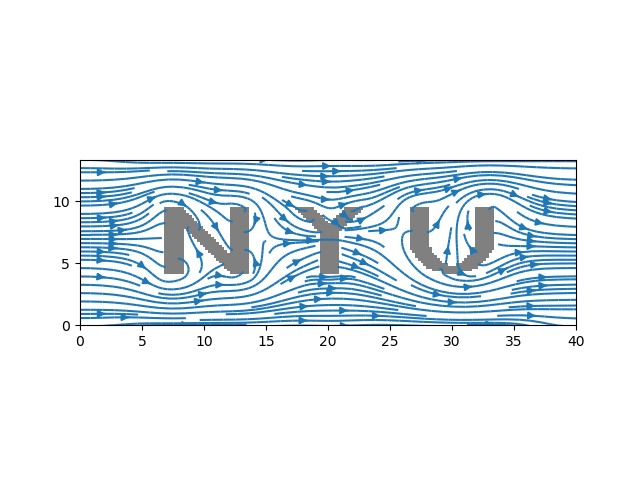
\includegraphics[width=10cm]{nyu.png}
\end{center}

As a proof of concept, the flow surrounding an object of complex shape was also simulated. The plot below shows the flow of a fluid around the block letters "NYU", embedded in the flow as no-slip boundaries. The resulting plot of the stream lines indicates a number of problems which need to be troubleshooted, but otherwise seems to display the expected behavior; i.e. velocity at the obstacle boundaries are small, and the flow generally runs tangent to the obstacles. To attain a better stream plot, it is necessary to use a more precise stream plot function, and to ensure that the fluid is not able to stream through boundaries which are only a few nodes thick. In particular, it is yet to be determined what resolution is needed to properly determine the flow in a "crevice" such as that formed by the "U". Furthermore, there is a node at the top of the "Y" which is surrounded by three boundary nodes; this type of boundary likely needs special treatment, and it is probably best to remove all such nodes from an embedded obstacle if possible. 

\section{Conclusion}
To summarize, we have discussed the theory underlying the standard Lattice Boltzmann Method, implemented a D2Q9 LBM in Python, and performed a number of simulations and calculations of flows subject to various boundary conditions. The simulation of a pressure-driven flow through a channel indicate that our model behaves appropriately, and suggests that the accuracy of the current implementation may be determined more rigorously through a series of benchmark tests in the incompressible limit. Furthermore, our results suggest that for straight walls, the MEM method provides an accurate means of force calculation. 

We have also shown that such an LBM implementation can model the flow around a cylinder with considerable accuracy, and exhibits the emergence of vortices at high Reynolds number consistent with theoretical predictions. We have also demonstrated the ability to model the flows around arbitrary geometries with decent accuracy. The main difficulties which hindered the implementation of complex boundary conditions were the loss of accuracy of the bounce-back method resulting from the introduction of curved boundaries, and problems which arose due to low resolution. However, the first of these issues can be overcome by the introduction of higher-order boundary methods which handle curved boundaries (which already exist and have been discussed), and parallellizing this code will drastically improve the resolution which we can reasonably calculate. Consequently, the LBM implementation which we have presented proves very promising for modeling flows around complex geometries.  

\bibliographystyle{unsrt}
\bibliography{mybib}





\end{document}
